\chapter{Methodology} \label{ch:methodology}

This chapter describes the architecture and methods that were needed in order to investigate the research questions presented in Section \ref{goals_and_research_questions}. An overview of the physical testbed will first be given, followed by the general setup for each machine and how the \gls{tcp} experimentation have been conducted using the tool \gls{teacup}. \todo{rework?}









\section{System Overview}

The objective of the system is to perform automated \gls{tcp} experiments in order to validate the reproducibility and significance of our results. This section aims to give a brief overview of the system as a whole and its individual components.




\subsection{The Raspberry Pi 3 Cluster}

The system consists of eight connected Raspberry Pi machines. The Raspberry Pi machine is a series of small single-board computers developed in the UK by the Raspberry Pi Foundation to promote teaching of basic computer science in schools and in developing countries. The Raspberry Pi 3 Model B+ was released in 2018, and is the model used in this cluster.

% \begin{table}[H]
%     \centering
%     \begin{tabular}{ |p{4cm}|p{2cm}|p{4cm}|p{2cm}|p{2cm}|  }
%         \hline
%         \multicolumn{5}{|c|}{\textbf{Raspberry Pi 3 Model B+ Specifications}} \\
%         \hline
%         \textbf{CPU} & \textbf{RAM} & \textbf{NICs} & \textbf{Storage} & \textbf{USB}\\
%         \hline
%         Broadcom BCM2837B0 \newline Cortex-A53 (ARMv8) 64-bit SoC \newline 1.4GHz, Quad-core &
%         1GB LPDDR2 SDRAM &
%         Gigabit Ethernet over USB 2.0 \newline Dual IEEE 802.11ac WiFi, Bluetooth 4.2 &
%         32GB Micro-SD &
%         4 USB 2.0 ports\\
%         \hline
%     \end{tabular}
%     \caption{The hardware specifications of Raspberry Pi 3 Model B+.}
% \end{table}

\begin{wraptable}{r}{5cm}
    \begin{tabular}{ |p{1cm}|p{3cm}| }
        \hline
        \multicolumn{2}{|c|}{\textbf{Raspberry Pi 3 Model B+}} \\
        \hline
        \textbf{CPU} & Broadcom BCM2837B0 \newline Cortex-A53 (ARMv8) 64-bit SoC 1.4GHz Quad-core \\
        \hline
        \textbf{RAM} & 1GB LPDDR2 SDRAM \\
        \hline
        \textbf{NICs} & Gigabit Ethernet over USB 2.0 \newline Dual IEEE 802.11ac WiFi, Bluetooth 4.2 \\
        \hline
        \textbf{FS} & 32GB Micro-SD \\
        \hline
        \textbf{USB} & 4 USB 2.0 ports \\
        \hline
    \end{tabular}
    \caption{Raspberry Pi 3 Model B+ hardware specifications.}
\end{wraptable}

All the machines are hooked up to a single Zyxel switch. The switch provides interconnectivity, and in addition powers the machines through \gls{poe}. \todo{more?}

\begin{figure}[H]
    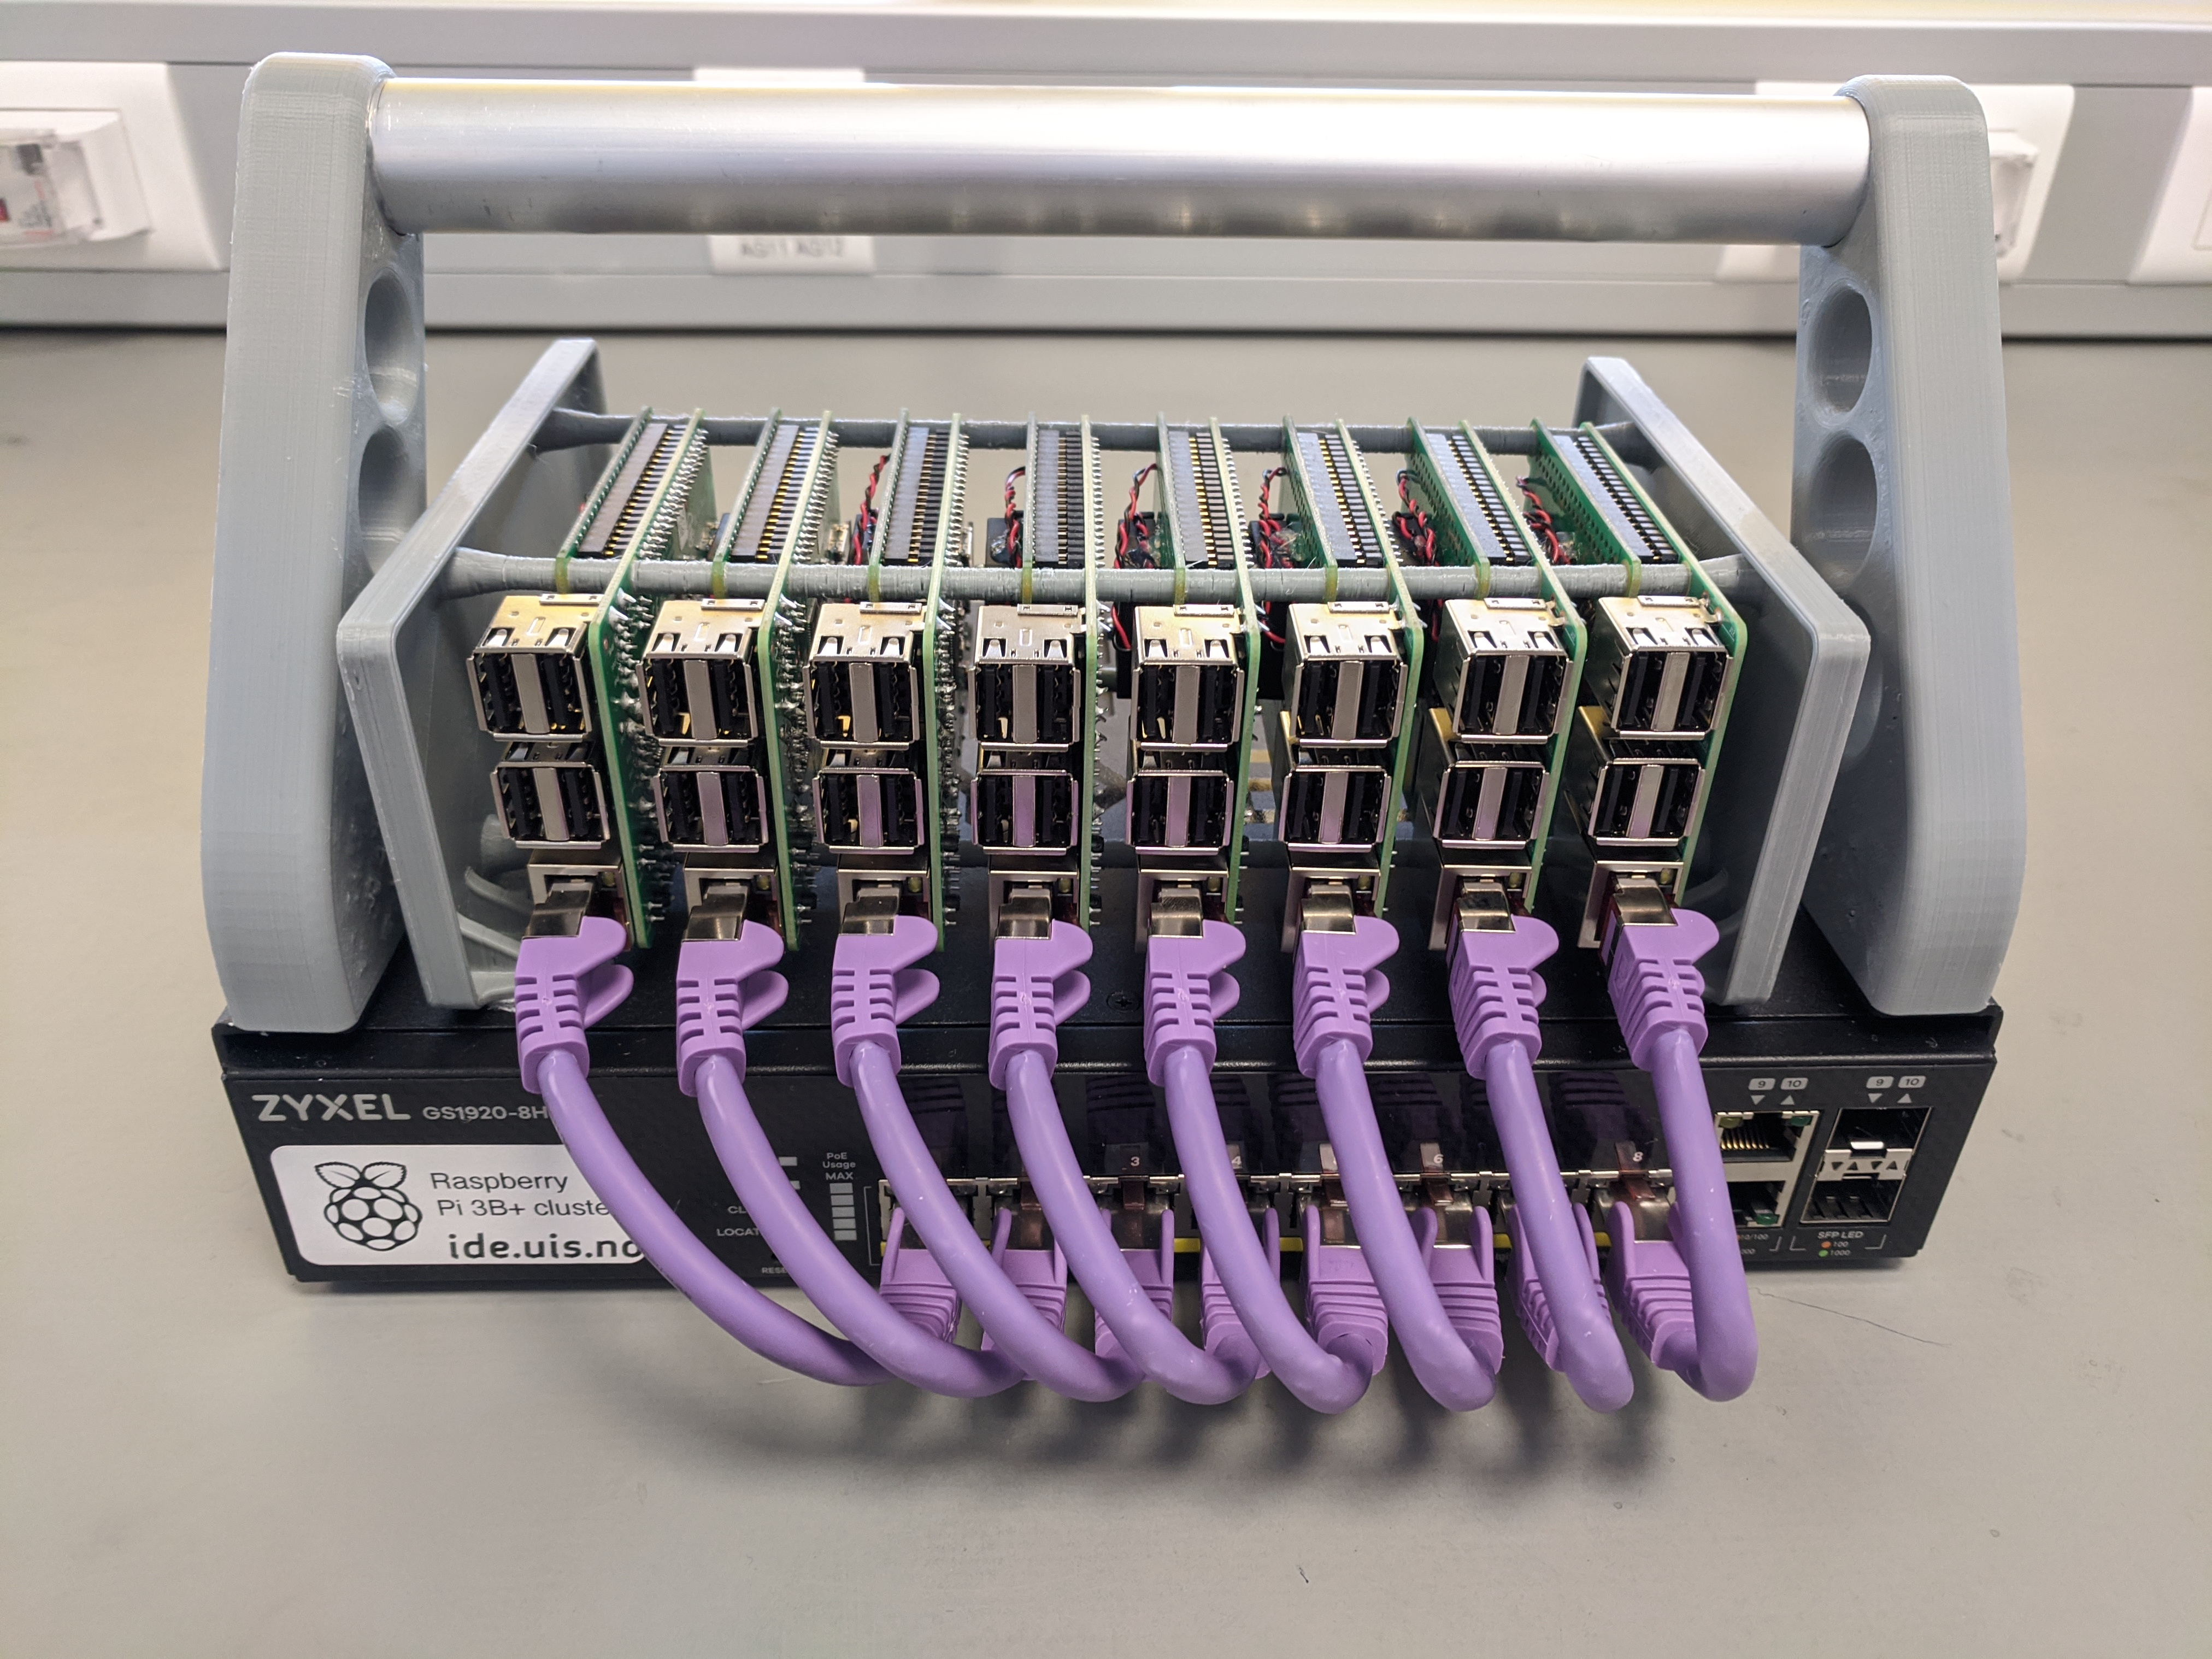
\includegraphics[width=0.55\linewidth]{pi3cluster}
    \captionsetup{width=1.0\linewidth,justification=raggedright,singlelinecheck=false}
    \caption{The Raspberry Pi 3B+ cluster all hooked to a Zyxel switch.}
    \label{fig:pi3cluster}
\end{figure}

% Fix wraptable bleeding
\clearpage




\subsection{Network Topology} \label{network_topology}

The testbed consists of two networks --- the \textit{controller} network in which all machines are connected directly, and the \textit{experimental} network separated by two subnets with a router in-between.

\begin{figure}[H]
    \centering
    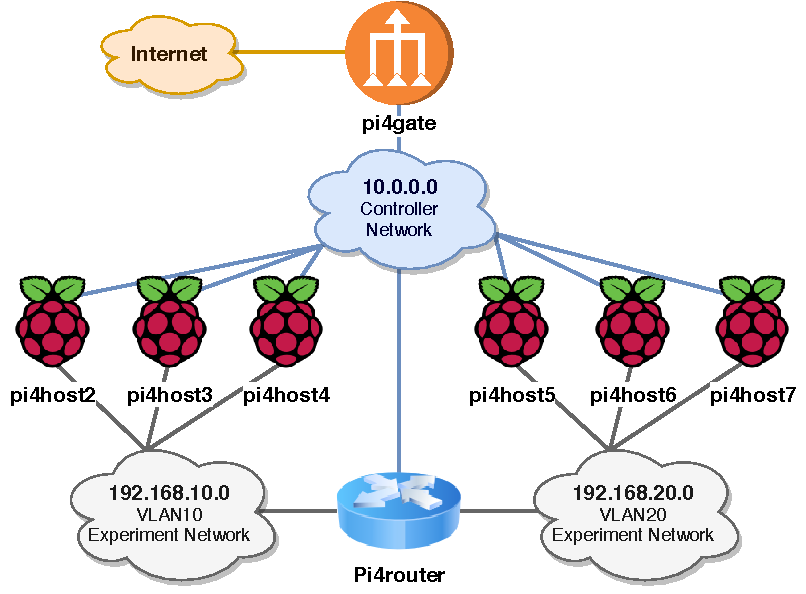
\includegraphics[width=0.6\linewidth]{network_topology}
    \captionsetup{width=0.6\linewidth}
    \caption{The logical network topology for the Raspberry Pi 3B+ cluster testbed.}
    \label{fig:network_topology}
\end{figure}

Since the entire testbed is connected to a single switch only, and each Raspberry Pi 3B+ machine has only one Ethernet interface, both \gls{vlan} and virtual interfaces have been used to achieve the desired network topology presented above. In addition, one USB-to-Ethernet adapter was necessary on the router in order to conduct network experimentation with \gls{teacup}. The \gls{vlan} setup on the switch is explained in Section \ref{zyxel} while the general network setup for every machine is explained in the remaining sections.

A summary table of the network setup for each machine follows.

\todo{restructure page}

\begin{table}[H]
    \centering
    \begin{tabular}{ |p{2cm}|p{6cm}|p{3cm}|  }
        \hline
        \multicolumn{3}{|c|}{\textbf{Summary Network Setup}} \\
        \hline
        \textbf{Hostname} & \textbf{IP address} & \textbf{OS}\\
        \hline
        pi3router & 10.0.1.1 --- eth0 \newline 172.16.10.1 --- eth0:10 (virtual) \newline 172.16.20.1 --- eth1 (USB-to-eth) & Raspbian Buster (Linux)\\
        \hline
        pi3host2 & 10.0.1.2 --- eth0 \newline 172.16.10.2 --- eth0:10 (virtual) & FreeBSD 12.1\\
        \hline
        pi3host3 & 10.0.1.3 --- eth0 \newline 172.16.10.3 --- eth0:10 (virtual) & FreeBSD 12.1\\
        \hline
        pi3host4 & 10.0.1.4 --- eth0 \newline 172.16.10.4 --- eth0:10 (virtual) & FreeBSD 12.1\\
        \hline
        pi3host5 & 10.0.1.5 --- eth0 \newline 172.16.20.5 --- eth0:20 (virtual) & FreeBSD 12.1\\
        \hline
        pi3host6 & 10.0.1.6 --- eth0 \newline 172.16.20.6 --- eth0:20 (virtual) & FreeBSD 12.1\\
        \hline
        pi3host7 & 10.0.1.7 --- eth0 \newline 172.16.20.7 --- eth0:20 (virtual) & FreeBSD 12.1\\
        \hline
        pi3gate & DHCP --- eth0 \newline 10.0.1.254 --- eth0:1 (virtual) & Raspbian Buster (Linux)\\
        \hline
    \end{tabular}
    \caption{The hostnames, IP addresses and OS for each Raspberry Pi 3B+ machine in the cluster.}
\end{table}

The table above lists the configured Raspberry Pi 3B+ machines in left to right order as seen from \ref{fig:pi3cluster}. That is, the left most machine is set up as the router, and the right most machine is set up as the gateway.




\subsection{Zyxel GS1920-8HP} \label{zyxel}

The Zyxel GS1920-8HP model is a managed switch with 10 available ports for interconnectivity. The Zyxel switch is what powers every Raspberry Pi 3B+ machine using \gls{poe}, with port 9 providing Internet access.

\begin{figure}[H]
    \centering
    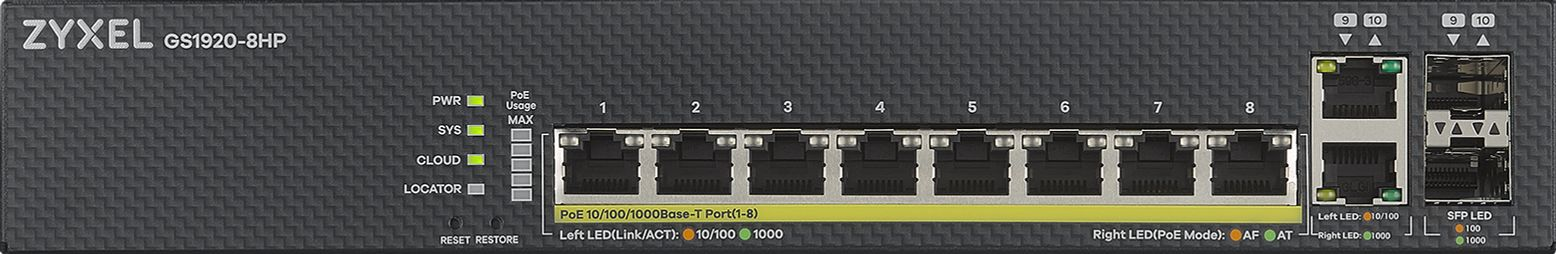
\includegraphics[width=1.0\linewidth]{zyxel}
    \captionsetup{width=1.0\linewidth}
    \caption{The front of the Zyxel GS1920-8HP managed switch.}
    \label{fig:zyxel}
\end{figure}

In order to logically separate two subnets on a single switch, as illustrated in \ref{fig:network_topology}, two \gls{vlan}s must be set up. This can easily be done through the switch's graphical user interface that can be accessed in several ways as shown in the official \href{https://www.zyxel.com/support/download_landing/product/gs1920_series_18.shtml?c=gb&l=en&pid=20130521174252&tab=Quick_Start_Guide&pname=GS1920%20Series}{quick start guide} \footnote{\url{https://www.zyxel.com/products_services/8-24-48-port-GbE-Smart-Managed-Switch-GS1920-Series}}. In short, connect a computer to the Zyxel switch with an Ethernet cable, set a static IP of 192.168.1.10, and access the graphical user interface in a web browser by visiting the address 192.168.1.1.

The default username and password for Zyxel GS1920-8HP is \lstinline{admin} and \lstinline{1234}, respectively. Once logged in, go to \lstinline{Advanced Application -> VLAN -> VLAN Configuration -> Static VLAN Setup}.

\begin{figure}[H]
    \centering
    \begin{subfigure}{0.5\linewidth}
        \centering
        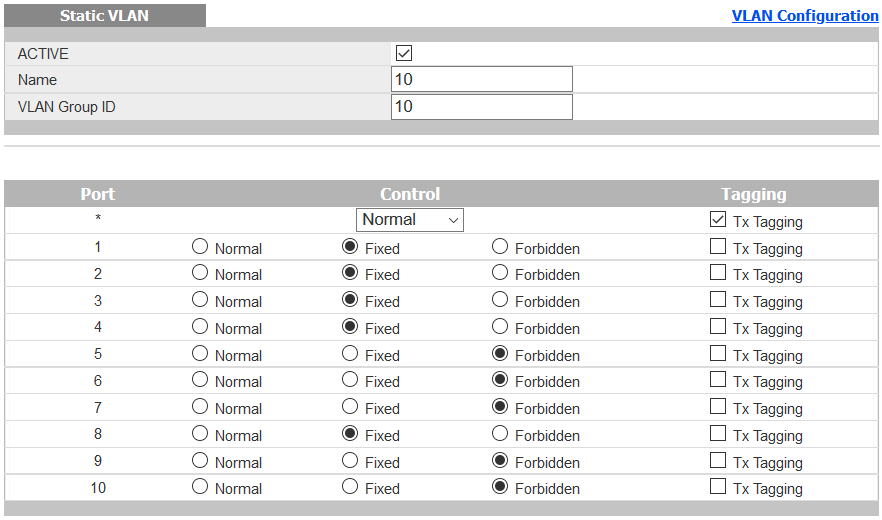
\includegraphics[width=1.0\linewidth]{vlan10}
        \caption{VLAN 10}
        \label{fig:vlan10}
    \end{subfigure}%
    \begin{subfigure}{0.5\linewidth}
        \centering
        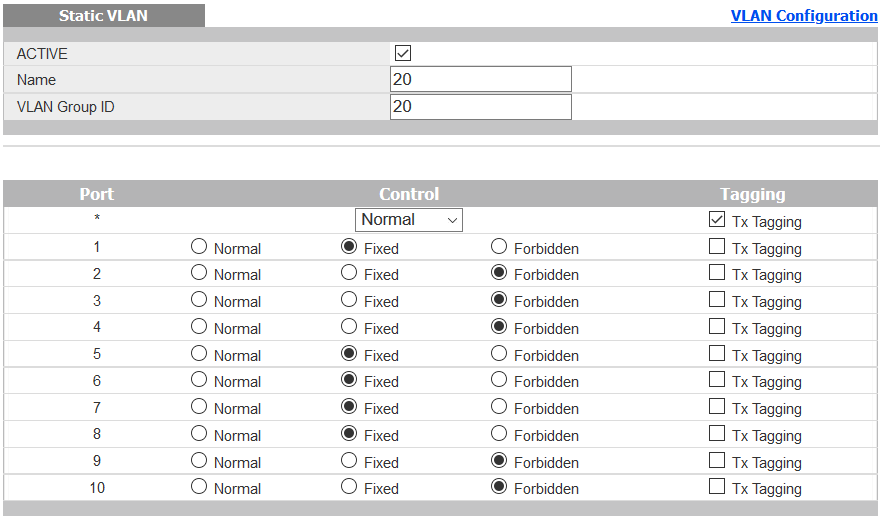
\includegraphics[width=1.0\linewidth]{vlan20}
        \caption{VLAN 20}
        \label{fig:vlan20}
    \end{subfigure}
    \caption{The configuration for the two \gls{vlan}s on Zyxel GS1920-8HP.}
    \label{fig:vlans}
\end{figure}

Create two \gls{vlan}s as shown above, confirming each creation with the \lstinline{Add} button. When done, persist the changes with the \lstinline{Save} button in the top right corner.









\section{General Setup}

This section serves as a guide for reproducing the general setup and configuration for the testbed. For the next sections, the following common tasks are assumed to have already been done on each Raspberry Pi 3B+ machine:

\begin{itemize}
    \item Installed an \gls{os} as specified in \ref{install_os}. Raspbian Buster is used on the gateway and router, and FreeBSD on the hosts.
    \item Changed the keyboard layout as specified in \ref{keyboard_layout}.
    \item Created a root user account as specified in \ref{root_account}.
    \item Updated the system as specified in \ref{update_system}.
    \item Enabled SSH as specified in \ref{enable_ssh}.
\end{itemize}

In addition, any given command is assumed to be run as \lstinline{root} user.




\subsection{Gateway}

This section describes how the machine with direct Internet access has been set up, known as the \textit{gateway}, and how it provides access and Internet for the other machines through \gls{nat}. The gateway is also known as the \textit{controller}, as this is where \gls{teacup} experiments are both configured and conducted from.


\subsubsection{Network}

The gateway is the only machine with direct Internet access through \gls{dhcp} on its main interface, with a virtual interface statically connected to the private controller network in order to communicate with the rest of the machines. To set up this, add the following to the \lstinline{/etc/network/interfaces} file:

\begin{minted}{bash}
# Main interface (Internet access)
auto eth0
iface eth0 inet dhcp

# Subinterface (controller-network)
auto eth0:1
iface eth0:1 inet static
address 10.0.1.254
netmask 255.255.255.0
\end{minted}

In order for the machines on the internal network to gain Internet access through the gateway, both \gls{ip} forwarding and \gls{nat} must be set up:

\begin{minted}{bash}
# Enable IP forwarding
echo 'net.ipv4.ip_forward=1' >> /etc/sysctl.conf

# NAT
update-alternatives --set iptables /usr/sbin/iptables-legacy
iptables -t nat -A POSTROUTING -o eth0 -j MASQUERADE
apt install iptables-persistent
\end{minted}

The hostname has also been changed to \lstinline{pi3gate} as specified in \ref{change_hostname}, followed by a reboot to apply all network changes.


\subsubsection{NTP Server}

\gls{teacup} requires that time is synchronized on all machines when running experiments. In order for the internal machines to synchronize their clock, an \gls{ntp} server must be set up. The gateway will provide this service, and is set up as specified in \ref{time_sync}.


\subsubsection{TEACUP} \label{teacup_gateway}

Every network experiment orchestrated by \gls{teacup} is initiated from the gateway, and so the majority of the tools for \gls{teacup} to work are installed on this machine. As described from the official \href{http://caia.swin.edu.au/tools/teacup/TEACUP-0.9_INSTALL.txt}{install} guide \footnote{\url{http://caia.swin.edu.au/tools/teacup/TEACUP-0.9_INSTALL.txt}}, with some slight adjustments, the following commands will install \gls{teacup} properly:

\todo{mention that TEACUP is 5 years old, and this is why the install steps had been slightly modified as Fabric has moved to Python 3}

\begin{minted}{bash}
# R
apt install -y r-base

# PDFJAM
apt install -y texlive-extra-utils

# SPP
apt install -y mercurial libpcap-dev build-essential
hg clone https://bitbucket.org/caia-swin/spp
cd spp
make
mkdir /usr/local/man/man1
make install
cd ..

# Fabric
apt install -y fabric python-pip python-dev libffi-dev libssl-dev
pip install fabric3
pip install -Iv pexpect==3.2

# TEACUP
wget https://sourceforge.net/projects/teacup/files/teacup-1.1.tar.gz
tar -xf teacup-1.1.tar.gz
\end{minted}

To verify that \gls{teacup} has been properly installed, a simple check can be done as follows:

\begin{minted}{bash}
mkdir experiment
cp teacup-1.1/example_configs/config-scenario1.py experiment/config.py
cp teacup-1.1/run.sh experiment/
cp teacup-1.1/fabfile.py experiment/
\end{minted}

Go into the \lstinline{experiment} folder and prepare to edit the \lstinline{config.py} file. Find the line containing \lstinline{TPCONF_script_path = '/home/teacup/teacup-0.8'} and change the \lstinline{path} to where you extracted \lstinline{teacup-1.1}. Finally, verify \gls{teacup} installation with the command \lstinline{fab check_config}. If no errors appear, all is good.


\subsubsection{Modifications to TEACUP}

Due to the restricted physical set up as shown in \ref{fig:pi3cluster} and discussed in \ref{network_topology}, virtual interfaces have been used extensively, particularly on the router. This introduced a conflict to the \gls{teacup} codebase, as it assigns a name to each interface before performing network logging with \lstinline{tcpdump}. However, this name is not unique since both the controller and experiment network shares the same interface, resulting in a \lstinline{duplicate handle error} from \gls{teacup}. A slight adjustment to the codebase was therefore necessary.

Applying the following "band-aid" to the \lstinline{loggers.py} file in \gls{teacup} should fix the error:

\begin{minted}{bash}
--- teacup-1.1/loggers.py
+++ teacup-1.1-modified/loggers.py
@@ -41,6 +41,7 @@
    from getfile import getfile
    from runbg import runbg
    
+   import random
    
    ## Collect all the arguments (here basically a dummy method because we
    ## dont used the return value)
@@ -505,7 +506,7 @@
                    snap_len, interface, file_name, tcpdump_filter)
        pid = runbg(tcpdump_cmd)
    
-       name = 'tcpdump-' + interface
+       name = 'tcpdump-' + interface + str(random.randint(0, 50000))
        #bgproc.register_proc(env.host_string, name, '0', pid, file_name)
        bgproc.register_proc_later(
            env.host_string,
\end{minted}

In additon, a few changes to the \lstinline{hostsetup.py} file in \gls{teacup} must be done. \gls{teacup} checks if the \lstinline{sysctl} variable \lstinline{net.inet.tcp.reass.overflows} exists, which it does not for the FreeBSD version that we are using. The default sender and receiver buffer on FreeBSD hosts must also be set to a higher value, otherwise experiments would experience a capped \gls{cwnd} value. The changes are easily done as follows:

\begin{minted}{bash}
--- teacup-1.1/hostsetup.py
+++ teacup-1.1-modified/hostsetup.py
@@ -858,7 +858,7 @@
 
     if htype == 'FreeBSD':
         # record the number of reassembly queue overflows
-        run('sysctl net.inet.tcp.reass.overflows')
+        #run('sysctl net.inet.tcp.reass.overflows')
 
         # disable auto-tuning of receive buffer
         run('sysctl net.inet.tcp.recvbuf_auto=0')
@@ -869,6 +869,8 @@
         # send and receiver buffer max (2MB by default on FreeBSD 9.2 anyway)
         run('sysctl net.inet.tcp.sendbuf_max=2097152')
         run('sysctl net.inet.tcp.recvbuf_max=2097152')
+        run('sysctl net.inet.tcp.recvspace=655360')
+        run('sysctl net.inet.tcp.sendspace=327680')
 
         # clear host cache quickly, otherwise successive TCP connections will
         # start with ssthresh and cwnd from the end of most recent tcp
\end{minted}

Finally, the tool \lstinline{spp} does not run on the Raspberry Pi 3 or ARM architecture at all, only displaying the helpful message "\lstinline{aborting}" when running it. TEACUP uses this tool to calculate \gls{rtt}, and fortunately is only needed when analyzing the results. In other words, the experiment data can easily be copied over to an x86 machine where \lstinline{spp} works, and then be analyzed from there. That is, follow the install instructions above from \ref{teacup_gateway} again as normal, but on an x86 machine instead.

\todo{custom aqm teacup changes}







\subsection{Router}

This section describes how the router has been set up. \todo{maybe expand...}


\subsubsection{Network}

The router serves as the intermediate device for the hosts in order to conduct more realistic experiments. The main interface is statically connected to the controller network, with two additional interfaces (one virtual and one USB-to-Ethernet) that function as the default gateway for the two separate subnets that the hosts reside in. To set the router up as such, add the following to the \lstinline{/etc/network/interfaces} file:

\begin{minted}{bash}
# Main interface (controller-network)
auto eth0
iface eth0 inet static
address 10.0.1.1
netmask 255.255.255.0
gateway 10.0.1.254

# Subinterface for VLAN 10 (experiment-network)
auto eth0:10
iface eth0:10 inet static
address 172.16.10.1
netmask 255.255.255.0
gateway 10.0.1.254

# USB-to-eth for VLAN 20 (experiment-network)
auto eth1
iface eth1 inet static
address 172.16.20.1
netmask 255.255.255.0
gateway 10.0.1.254
\end{minted}

In order for the hosts to communicate through the router, \gls{ip} forwarding must be enabled:

\begin{minted}{bash}
# Enable IP forwarding
echo 'net.ipv4.ip_forward=1' >> /etc/sysctl.conf
\end{minted}

The hostname has also been changed to \lstinline{pi3router} as specified in \ref{change_hostname}, followed by a reboot to apply all network changes.


\subsubsection{NTP Client}

To synchronize time for the router against the gateway, set the router up as an \gls{ntp} client as specified in \ref{time_sync}.


\subsubsection{TEACUP}

The router only needs two tools for \gls{teacup} to work properly when controlled from the gateway, and that is \lstinline{tcpdump} and \lstinline{ntp}:

\begin{minted}{bash}
# TEACUP tools on router
apt install -y tcpdump ntp
\end{minted}



\subsection{Hosts}

This section describes how each host has been set up. \todo{maybe expand...}


\subsubsection{Network}

The hosts are separated into two subnets. Hosts 2, 3 and 4 are on the network 172.16.10.0/24 (VLAN 10), while hosts 5, 6 and 7 are on 172.16.20.0/24 (VLAN 20). The main interface on each host is statically connected to the controller network, with an additional virtual interface (or \textit{alias} in FreeBSD) statically connected to the experimental network. To set up each host, run the following, but replace \lstinline{yy} with the appropriate \gls{vlan} and \lstinline{x} with the correct host number as illustrated in \ref{network_topology}:

\begin{minted}{bash}
# Main interface (controller-network)
echo 'ifconfig_ue0="inet 10.0.1.x netmask 255.255.255.0"' >> /etc/rc.conf
echo 'defaultrouter="10.0.1.254"' >> /etc/rc.conf

# Alias (experiment-network)
echo 'ifconfig_ue0_alias0="inet 172.16.yy.x netmask 255.255.255.0"' >> /etc/rc.conf
\end{minted}

In order for the hosts to communicate between each subnet, a static route must be added. Run the following to do so:

\begin{minted}{bash}
# Static route
echo 'static_routes="intnet"' >> /etc/rc.conf
echo 'route_intnet="-net 172.16.yy.0/24 172.16.xx.1"' >> /etc/rc.conf
\end{minted}

Replace \lstinline{yy} with the destination \gls{vlan} and \lstinline{xx} with the source \gls{vlan}.

The hostname has also been changed to \lstinline{pi3hostX} as specified in \ref{change_hostname}, where \lstinline{X} refers to the correct host number. A reboot will apply all network changes.


\subsubsection{NTP Client}

To synchronize time for each host against the gateway, set up each host as an \gls{ntp} client as specified in \ref{time_sync}.


\subsubsection{TEACUP}

\gls{teacup} requires four tools that must be installed on each host in order to run experiments, namely \lstinline{lighttpd},  \lstinline{iperf}, \lstinline{httperf} and \lstinline{nttcp}. The \lstinline{lighttpd} tool can be installed from the package repository with \lstinline{pkg install lighttpd}. A modified version of \lstinline{iperf} is used, and so must be installed from source as follows:

\begin{minted}{bash}
# Installing modified iperf on FreeBSD
wget https://sourceforge.net/projects/iperf2/files/iperf-2.0.9.tar.gz --no-check-certificate
tar -xf iperf-2.0.9.tar.gz
cd iperf-2.0.9
patch -p1 < iperf-2.0.9.patch
./configure
make
make install
\end{minted}

\todo{iperf-2.0.9.patch needs more explaining}

A modified version of \lstinline{httperf} is also used, but installing from source has proven unsuccessful. Thus, an unmodified version is therefore installed with \lstinline{pkg install httperf}. The last tool to install, \lstinline{nttcp}, is also modified, and so must be installed from source as follows:

\begin{minted}{bash}
# Installing modified nttcp on FreeBSD
wget http://caia.swin.edu.au/tools/teacup/downloads/nttcp-1.47-mod.tar.gz
tar -xf nttcp-1.47-mod.tar.gz
cd nttcp-1.47-mod
make
cp nttcp /bin/
\end{minted}









\section{TCP Experimentation with TEACUP}

\glsfirst{teacup} \footnote{\url{http://caia.swin.edu.au/tools/teacup}} is a software tool for running automated \gls{tcp} experiments in a controlled physical tested. It was made as a research project by \gls{caia} in 2005 to gain a better understanding of the impact of different \gls{cc} algorithms on \gls{tcp}-based streaming flows. \cite{teacup} The typical use-case involves a classical dumbbell topology where multiple hosts are connected on opposite sides of a bottleneck router. An essential part of the tool is the \textit{control host} or \textit{gateway} as we refer to it, which is where \gls{teacup} itself runs and orchestrates the configuration of the end hosts and bottleneck router before a particular experiment is conducted.

The process of installing and setting up \gls{teacup} is quite extensive. We experienced a lot of trouble \remark{problems?} due to the ARM architecture on Raspberry Pi as discussed in Section \todo{reference}. However, the effort was well worth it. We ended up with a single \gls{os} on each machine, where the hosts are running FreeBSD and the router and gateway are running Raspbian Buster (Linux). With a single configuration file (see Appendix \ref{teacup_gateway}), \gls{teacup} is able to perform experiments with multiple permuations --- traffic generation (such as \gls{tcp} bulk transfer), traffic shaping (such as bandwidth, delay and loss), traffic control (scheduling of packets with \gls{aqm}) and executing custom host commands such as enabling \gls{ecn}.

For each experiment, \gls{teacup} will collect a variety of metadata from the end hosts and bottleneck router. The resulting experiment data is then analyzed in order to generate graphical plots that can show either the throughput, \gls{rtt} (including smoothed) or \gls{cwnd} over time. The use of \gls{teacup} in our thesis serves to validate the results from our work, as every plot illustrated in Chapter \ref{evaluation} has been generated by it.

\todo{more?}









\section{Congestion Control in FreeBSD} \label{sec:cc_in_freebsd}

The FreeBSD networking stack saw a major enhancement with the release of version 9.0 --- modular congestion control was added, allowing \gls{cc} algorithms to be implemented as loadable kernel modules. The framework is referred to as \lstinline{mod_cc} \footnote{\url{https://www.freebsd.org/cgi/man.cgi?query=mod_cc&sektion=4&apropos=0&manpath=FreeBSD+12.1-RELEASE}}, and was the result of a research project called NewTCP from \gls{caia} that began in 2005. It initially focused on independent, interoperable implementations of new "high speed" \gls{tcp} \gls{cc} algorithms in FreeBSD, and eventually received FreeBSD Foundation support in order to port its modular congestion control framework and five congestion control algorithms into the official FreeBSD tree. \footnote{\url{http://caia.swin.edu.au/urp/newtcp}}

The available \gls{cc} algorithms on FreeBSD can be listed with the following command:

\begin{minted}{bash}
# Show available CC algorithms on FreeBSD
sysctl net.inet.tcp.cc.available
\end{minted}
By default, only NewReno is available. For others to be available, they must first be loaded with the dynamic kernel linker facility (\lstinline{kld}):

\begin{minted}{bash}
# Load FreeBSD CC module with kld
kldload cc_cubic
\end{minted}
FreeBSD comes with several \gls{cc} kernel modules. They reside in \lstinline{/boot/kernel} with the prefix \lstinline{cc_}. On our system, the following modules (\lstinline{.ko}-files) are found by default on the hosts:

\begin{minted}{bash}
# Output of 'ls /boot/kernel | grep cc_' on FreeBSD 12.1-RELEASE:
cc_cdg.ko
cc_chd.ko
cc_cubic.ko
cc_dctcp.ko
cc_hd.ko
cc_htcp.ko
cc_vegas.ko
\end{minted}
Once a \gls{cc} module has been loaded, it will show up as available and can be selected with:

\begin{minted}{bash}
# Select which CC algorithm to use on FreeBSD
sysctl net.inet.tcp.cc.algorithm=cubic
\end{minted}
In order to compile a FreeBSD kernel module, the kernel source is needed. The source must reflect the current installed system, which in our case means that it can be fetched as follows:

\begin{minted}{bash}
# Get FreeBSD kernel source
VERSION=12.1-RELEASE
ARCHITECTURE=arm64
fetch ftp://ftp.freebsd.org/pub/FreeBSD/releases/$ARCHITECTURE/$VERSION/src.txz
tar -C / -xzvf src.txz
\end{minted}
With the kernel source in place, the implementation code for existing \gls{cc} modules on FreeBSD can be found in \lstinline{/usr/src/sys/netinet/cc} with its corresponding \lstinline{Makefile} in \lstinline{/usr/src/sys/modules/cc} in order to build it.

The \lstinline{mod_cc} framework consists of the header file \lstinline{cc.h} and implementation file \lstinline{cc.c}. Once included in a kernel module, a set of hook functions becomes available that are called in various \gls{tcp} events. These functions are encapsulated in a \lstinline{cc_algo} structure in \lstinline{cc.h}, and together represent a congestion control algorithm in FreeBSD.

\begin{code}
\file{hook functions in cc.h}
\begin{minted}{c}
/*
 * Structure to hold data and function pointers that together represent a
 * congestion control algorithm.
 */
struct cc_algo {
    /* The name that uniquely identifies the algorithm */
    char name[TCP_CA_NAME_MAX];
    /* Init global module state on kldload. */
    int	(*mod_init)(void);
    /* Cleanup global module state on kldunload. */
    int (*mod_destroy)(void);
    /* Init CC state for a new control block. */
    int	(*cb_init)(struct cc_var *ccv);
    /* Cleanup CC state for a terminating control block. */
    void (*cb_destroy)(struct cc_var *ccv);
    /* Init variables for a newly established connection. */
    void (*conn_init)(struct cc_var *ccv);
    /* Called on receipt of an ack. */
    void (*ack_received)(struct cc_var *ccv, uint16_t type);
    /* Called on detection of a congestion signal. */
    void (*cong_signal)(struct cc_var *ccv, uint32_t type);
    /* Called after exiting congestion recovery. */
    void (*post_recovery)(struct cc_var *ccv);
    /* Called when data transfer resumes after an idle period. */
    void (*after_idle)(struct cc_var *ccv);
    /* Called for an additional ECN processing apart from RFC3168. */
    void (*ecnpkt_handler)(struct cc_var *ccv);
    /* Called for {get|set}sockopt() on a TCP socket with TCP_CCALGOOPT. */
    int (*ctl_output)(struct cc_var *, struct sockopt *, void *);
    /* Macro that declares a structure that connects the elements in the tail queue. */
    STAILQ_ENTRY (cc_algo) entries;
};
\end{minted}
\captionof{listing}{An excerpt from \lstinline{cc.h} showing the set of hook functions that allows congestion control algorithms to be implemented as a dynamically loadable kernel module in FreeBSD.}
\label{code:freebsd-cc}
\end{code}

Any \lstinline{mod_cc} module must instantiate the \lstinline{cc_algo} structure, but only the \lstinline{name} field is required to be defined. The instantiation is provided by the \lstinline{DECLARE_CC_MODULE(ccname, &ccalgo)} macro used to register a module with the \lstinline{cc_mod} framework, where \lstinline{ccname} specifies the name of the module, and \lstinline{&ccalgo} points to a structure containing the function pointer assignments for the hook functions. A simple example follows.

\begin{code}
\file{simple mod\_cc example}
\begin{minted}{c}
#include <sys/param.h>
#include <sys/kernel.h>
#include <sys/malloc.h>
#include <sys/module.h>
#include <sys/socket.h>
#include <sys/socketvar.h>
#include <sys/sysctl.h>
#include <sys/systm.h>
#include <net/vnet.h>
#include <netinet/tcp.h>
#include <netinet/tcp_seq.h>
#include <netinet/tcp_var.h>
#include <netinet/cc/cc.h>
#include <netinet/cc/cc_module.h>

/* Define functions to be used. */
static int example_mod_init(void);
static int example_mod_destroy(void);

/* Assign name and hook functions to the defined above. */
struct cc_algo example_cc_algo = {
    .name = "example",
    .mod_init = example_mod_init,
    .mod_destroy = example_mod_destroy
};

/* Private struct with members that can be used throughout the module. */
struct example {
    uint32_t value;
};

/* Implementation of the mod_init hook function. */
static int example_mod_init(void) {
    printf("Hello, world!\n");
    return (0);
}

/* Implementation of the mod_destroy hook function. */
static int example_mod_destroy(void) {
    printf("Goodbye, world!\n");
    return (0);
}

/* Register module to the cc_mod framework and instantiate example_cc_algo struct. */
DECLARE_CC_MODULE(example, &example_cc_algo);
\end{minted}
\captionof{listing}{A simple \lstinline{mod_cc} module example where the \lstinline{name}, \lstinline{mod_init} and \lstinline{mod_destroy} have been defined. The module simply prints "Hello, world!" when loaded, and "Goodbye, world!" when unloaded, which can be viewed with the command \lstinline{dmesg}.}
\label{code:freebsd-cc}
\end{code}

To access \gls{tcp} related variables, the macro \lstinline{CCV(ccv, what)} is used, where \lstinline{ccv} points to the \lstinline{cc_var} structure defined in \lstinline{cc.h} (passed by many hook functions from \ref{code:freebsd-cc}), and \lstinline{what} refers to the variable to be retrieved. For instance, the call \lstinline{CCV(ccv, snd_cwnd)} will return the current \gls{cwnd}. For complete examples of \gls{cc} kernel modules in FreeBSD, see Appendix \ref{app:freebsd_cc_modules}.









\section{Achieving Low Latency with ABE}

Since \gls{abe} is already in mainline FreeBSD kernel, \cite{rfc8511} and the hosts in our testbed are running FreeBSD, it is only a matter of enabling it with the following command:

\begin{minted}{bash}
# Enabling ABE on FreeBSD
sysctl net.inet.tcp.cc.abe=1
\end{minted}
NewReno in FreeBSD utilizes the \gls{aimd} feedback control algorithm for adjusting the \gls{cwnd}, meaning that it grows linearly when in congestion avoidance, and experiences an exponential reduction when congestion is detected. The multiplicative decrease factor is specified as a percentage, and can be changed with the following commands:

\begin{minted}{bash}
# Set multiplicative window decrease factor in FreeBSD for lossy signaling (default 50)
sysctl net.inet.tcp.cc.newreno.beta=50

# Set multiplicative window decrease factor in FreeBSD for ECN signaling (default 80)
sysctl net.inet.tcp.cc.newreno.beta_ecn=80
\end{minted}
Upon a congestion signal with \gls{abe} enabled, the static reduction factor in NewReno is updated as follows:

\begin{minted}{c}
static void newreno_cong_signal(struct cc_var *ccv, uint32_t type) {
    /* ... */
    if (V_cc_do_abe && type == CC_ECN)
        factor = beta_ecn; /* factor if ECN */
    else
        factor = beta; /* factor if loss */
    /* ... */
    cwin = max(((uint64_t)cwin * (uint64_t)factor) / (100ULL * (uint64_t)mss), 2) * mss;
\end{minted}
The new \gls{cwnd} calculation follows the multiplicative part of the \gls{aimd} scheme from \ref{eq:aimd}, which effectively becomes

\begin{equation} \label{eq:cwnd_newreno}
    \mathrm{cwnd} = \begin{cases}
        \mathrm{cwnd} \times 50/100, & \text{if loss},\\
        \mathrm{cwnd} \times 80/100, & \text{if ECN}
    \end{cases}
\end{equation}

where cwnd is the current \gls{cwnd}. The resulting value is then scaled up by the \glsfirst{mss} to get the amount in bytes. Finally, the result is applied in a \lstinline{switch} statement where either only the \gls{ssthresh} is set in the case of a timeout, or both the \gls{ssthresh} and current \gls{cwnd} is set in the case of \gls{ecn}:

\begin{minted}{c}
case CC_NDUPACK: /* packet loss or timeout */
    if (!IN_FASTRECOVERY(CCV(ccv, t_flags))) {
        /* ... */
        if (!IN_CONGRECOVERY(CCV(ccv, t_flags)))
            CCV(ccv, snd_ssthresh) = cwin;
        ENTER_RECOVERY(CCV(ccv, t_flags));
    }
    break;
case CC_ECN: /* ECN */
    if (!IN_CONGRECOVERY(CCV(ccv, t_flags))) {
        CCV(ccv, snd_ssthresh) = cwin;
        CCV(ccv, snd_cwnd) = cwin;
        ENTER_CONGRECOVERY(CCV(ccv, t_flags));
    }
    break;
\end{minted}
The complete implementation details for NewReno can be found in Appendix \ref{cc_newreno}.









\section{Dynamic Alternative Backoff with ECN}

\glsfirst{dabe} represents our work that builds upon \gls{abe}. Instead of reducing the \gls{cwnd} by a constant factor in the event of an \gls{ecn} congestion signal, we reduce by the ratio of the shortest \gls{rtt} measured and the most recent one. Hence, if the \gls{rtt} rises, the resulting backoff is also greater, but if the \gls{rtt} remains stable, the backoff is less. The shortest, or \textit{minimum}, \gls{rtt} serves as the optimal point in which the network experiences no congestion.

\begin{figure}[H]
    \centering
    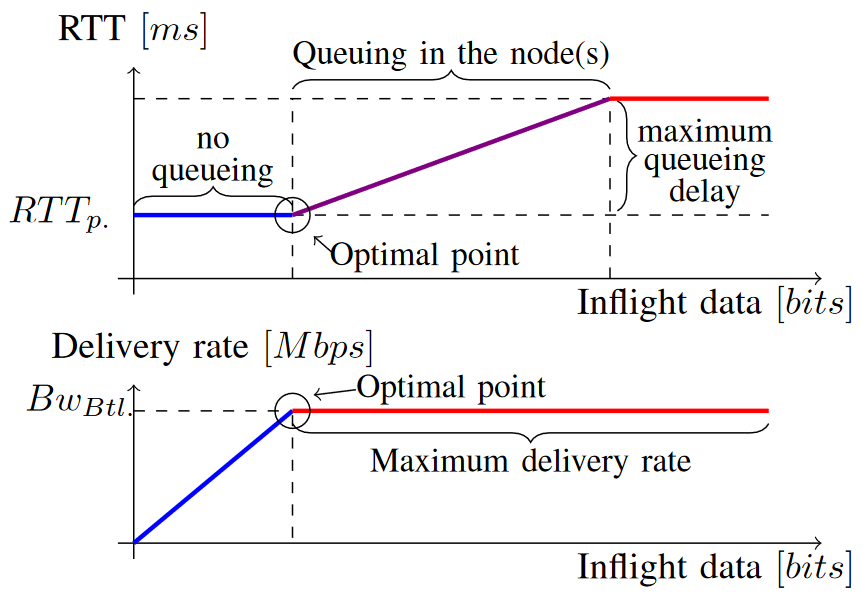
\includegraphics[width=0.6\linewidth]{rtt_queue}
    \captionsetup{width=0.6\linewidth}
    \caption{The effect on the \gls{rtt} when buffers start to fill and queues are formed. \todo{update image}}
    \label{fig:rtt_queue}
\end{figure}

% \begin{wrapfigure}{r}{0.5\textwidth}
%     \centering
%     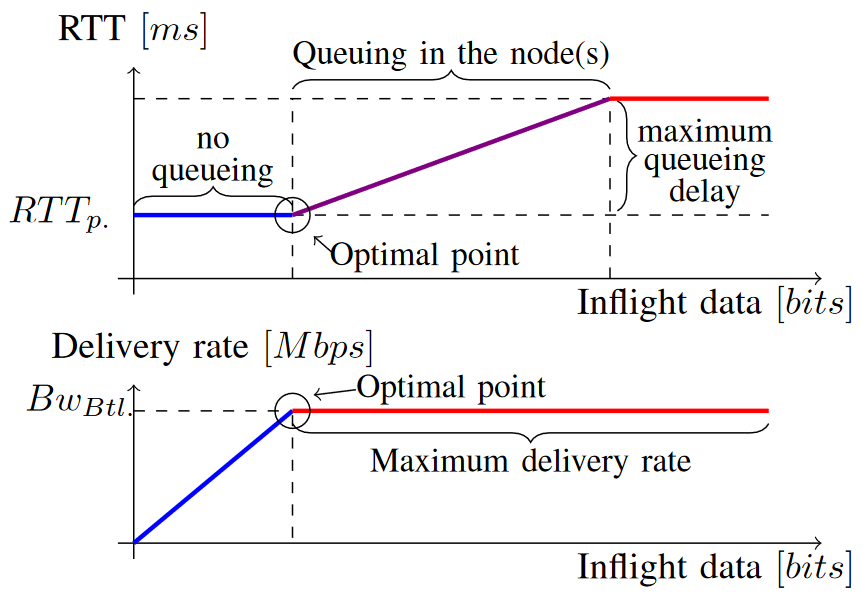
\includegraphics[width=0.5\textwidth]{rtt_queue}
%     \captionsetup{width=0.5\linewidth}
%     \caption{The effect on the \gls{rtt} when buffers start to fill and queues are formed. \todo{update image}}
% \end{wrapfigure}

Our work follows \gls{abe}'s spirit in that it is a simple sender-side only modification. In essence, we are only updating the \gls{ecn} congestion response. From the multiplicative part of the \gls{aimd} scheme from \ref{eq:aimd}, the new \gls{cwnd} value now becomes

\begin{equation} \label{eq:cwnd_improved_abe}
    \mathrm{cwnd} = \begin{cases}
        \mathrm{cwnd} \times 0.5, & \text{if loss},\\
        \mathrm{cwnd} \times \dfrac{\mathrm{RTT}_{min}}{\mathrm{RTT}}, & \text{if ECN}
    \end{cases}
\end{equation}

where $\mathrm{RTT}_{min}$ is the minimum \gls{rtt} that has been measured and is continually updated, and the $\mathrm{RTT}$ is the most recent measure. In order to implement this, we need \gls{rtt} measurements. This is true for any delay-based \gls{cc} algorithm, and so FreeBSD comes included with such functionality --- the Enhanced	Round Trip Time (ERTT) \textit{Khelp} module, referred to as \lstinline{h_ertt} \footnote{\url{https://www.freebsd.org/cgi/man.cgi?query=h_ertt&apropos=0&sektion=4&manpath=FreeBSD+12.1-RELEASE}}. \lstinline{Khelp} is another kernel framework in FreeBSD with the aim to provide a structured way to dynamically extend the kernel at runtime. The \lstinline{h_ertt} works within the \lstinline{khelp} framework to provide for enhanced \gls{rtt} estimates for all new \gls{tcp} connections created after the time at which the \gls{cc} module was loaded. Both \lstinline{khelp} and its \lstinline{h_ertt} module first appeared in FreeBSD 9.0, made by the same people who worked on the NewTCP research project which brought modular congestion control to FreeBSD.

The \lstinline{h_ertt} module provides several key pieces of data. In particular for us is the most \textit{recent} \gls{rtt} measurement and the \textit{shortest} \gls{rtt} measurement that has been taken.

\begin{code}
\file{the ertt structure}
\begin{minted}{c}
/* Structure used as the ertt data block. */
struct ertt {
    /* Information about transmitted segments to aid in RTT calculation. (Private) */
    TAILQ_HEAD(txseginfo_head, txseginfo) txsegi_q;
    /* Bytes TX so far in marked RTT. (Private) */
    long bytes_tx_in_rtt;
    /* Final version of above. */
    long bytes_tx_in_marked_rtt;
    /* cwnd for marked RTT. */
    unsigned long marked_snd_cwnd;
    /* Per-packet measured RTT. */
    int	rtt;
    /* Maximum RTT measured. */
    int	maxrtt;
    /* Minimum RTT measured. */
    int	minrtt;
    /* Guess if the receiver is using delayed ack. (Private) */
    int	dlyack_rx;
    /* Keep track of inconsistencies in packet timestamps. (Private) */
    int	timestamp_errors;
    /* RTT for a marked packet. (Private) */
    int	markedpkt_rtt;
    /* Flags to signal conditions between hook function calls. */
    uint32_t flags;
};
\end{minted}
\captionof{listing}{An excerpt from \lstinline{h_ertt.h} showing the fields for the \lstinline{ertt} structure that is associated with each \gls{tcp} connection. The private fields should not be manipulated by any code	outside of the \lstinline{h_ertt} implementation.}
\label{code:ertt.h}
\end{code}

To make the \lstinline{h_ertt} module available, the header files \lstinline{khelp.h} and \lstinline{h_ertt.h} must be included. To access the data from \lstinline{h_ertt}, a unique ID must be generated and used. In addition, we must specify that the \gls{cc} algorithm now depends on another module, which is done with the \lstinline{MODULE_DEPEND(name, moddepend, int minversion, int prefversion, int maxversion)} macro. The implementation for this follows.

\begin{minted}{c}
#include <sys/khelp.h>
#include <netinet/khelp/h_ertt.h>
/* ... */
static int32_t ertt_id;
/* ... */
static int newreno_dabe_init(void) {
	ertt_id = khelp_get_id("ertt");
	if (ertt_id <= 0) {
		printf("%s: h_ertt module not found\n", __func__);
		return (ENOENT);
	}
	return (0);
}
/* ... */
MODULE_DEPEND(newreno_abe, ertt, 1, 1, 1);
\end{minted}
The \lstinline{h_ertt} module is then used to fetch the minimum and most recent \gls{rtt} in order to calculate the new \gls{cwnd} from \ref{eq:cwnd_improved_abe} in the event of an \gls{ecn} congestion signal. The implementation for this follows.

\begin{minted}{c}
static void newreno_abe_cong_signal(struct cc_var *ccv, uint32_t type) {
    /* ... */
    struct ertt *e_t = khelp_get_osd(CCV(ccv, osd), ertt_id);
    /* ... */
    switch (type) {
    /* ... */
    case CC_ECN:
        if (!IN_CONGRECOVERY(CCV(ccv, t_flags))) {
            CCV(ccv, snd_ssthresh) = CCV(ccv, snd_cwnd) * e_t->minrtt / e_t->rtt;
            CCV(ccv, snd_cwnd) = CCV(ccv, snd_ssthresh);
            ENTER_CONGRECOVERY(CCV(ccv, t_flags));
        }
        break;
    }
}
\end{minted}
The \lstinline{CCV(ccv, snd_cwnd)} call fetches the current \gls{cwnd}, and gets multiplied by \lstinline{e_t->minrtt / e_t->rtt} which is the ratio of the minimum \gls{rtt} and most recent \gls{rtt} provided by the \lstinline{h_ertt} module.